% ============================================================
%  Physics of Learning — Chapter 1: Mathematical Foundations
%  Tufte-handout format with TikZ figures
% ============================================================
\documentclass[justified,notoc]{tufte-handout}

% ---------- mathematics ----------
\usepackage{amsmath,amssymb,amsfonts,mathrsfs,bm}

% ---------- graphics ----------
\usepackage{tikz,pgfplots}
\pgfplotsset{compat=1.18}
\usetikzlibrary{
  arrows.meta,
  decorations.pathreplacing,
  decorations.markings,
  positioning,
  calc,
  patterns,
  shapes.geometric,
  intersections,
  fillbetween
}
\usepgfplotslibrary{fillbetween,groupplots}

% ---------- layout & colour ----------
\usepackage{xcolor,microtype,booktabs,enumitem}
\usepackage[most]{tcolorbox}
\tcbuselibrary{theorems}

% ---------- hyperref (tufte loads it; just set colours) ----------
\hypersetup{
  colorlinks=true,
  linkcolor=black!60,
  urlcolor=black!60,
  citecolor=black!60
}

% ---------- colours ----------
\definecolor{tuftered}{RGB}{179,27,27}
\definecolor{tufteblue}{RGB}{28,80,150}
\definecolor{resultbox}{RGB}{245,245,240}
\definecolor{resultframe}{RGB}{160,140,100}

% ---------- boxed results (Tufte-width) ----------
\newtcolorbox{keyresult}{
  colback=resultbox,
  colframe=resultframe,
  boxrule=0.6pt,
  arc=2pt,
  left=6pt, right=6pt, top=4pt, bottom=4pt
}

% ---------- macros ----------
\def\d{\mathrm{d}}
\def\E{\mathbb{E}}
\def\R{\mathbb{R}}
\def\N{\mathcal{N}}
\def\var{\mathrm{Var}}
\def\P{\mathbb{P}}
\renewcommand{\vec}[1]{\mathbf{#1}}

% ---------- pgfplots base style ----------
\pgfplotsset{
  tufte axis/.style={
    width=\linewidth,
    height=0.72\linewidth,
    axis line style={thin, black!70},
    tick style={thin, black!60},
    tick label style={font=\small},
    label style={font=\small},
    title style={font=\small\bfseries},
    grid=major,
    grid style={dotted,black!20},
    minor tick num=1,
  }
}

% ============================================================
\title{Mathematical Foundations}
\author{S~Ganga~Prasath \& Kannabiran~Seshasayanan}
\date{Physics of Learning · IIT Madras}
% ============================================================

\begin{document}
\maketitle

\begin{abstract}
\noindent
These notes develop the core mathematical toolkit for the course: the language of probability, three generating functions (MGF, CGF, characteristic function), Gaussian integration in arbitrary dimension, Wick's theorem, the saddle-point approximation, and the Hubbard--Stratonovich transformation. Every definition is followed by a worked example; every theorem is derived step by step.
\end{abstract}

% ============================================================
\section{Probability: basic definitions}
% ============================================================

\newthought{A \textbf{sample space}} $\Omega$ is the set of all possible outcomes of an experiment. A \textbf{random variable} $X$ is a function $X:\Omega\to\mathbb{R}$ assigning a real number to each outcome. When $X$ is continuous its distribution is described by a \textbf{probability density function} (pdf) $f_X(x)$ satisfying
\begin{equation}
  f_X(x)\geq 0, \qquad \int_{-\infty}^{\infty} f_X(x)\,\d x = 1.
\end{equation}
The probability that $X$ falls in $[a,b]$ is $\P(a\leq X\leq b)=\int_a^b f_X(x)\,\d x$. The \textbf{cumulative distribution function} (CDF) is $F_X(x)=\int_{-\infty}^x f_X(t)\,\d t$, so $f_X=F_X'$. When $X$ is discrete we write $P(X=x_k)=p_k$ with $\sum_k p_k=1$.

The \textbf{expectation} and \textbf{variance} are
\begin{equation}
  \E[X]=\int_{-\infty}^{\infty} x\,f_X(x)\,\d x, \qquad
  \var(X)=\E[X^2]-(\E[X])^2.
\end{equation}

% ---- figure: five distribution shapes ----
\begin{figure*}
\centering
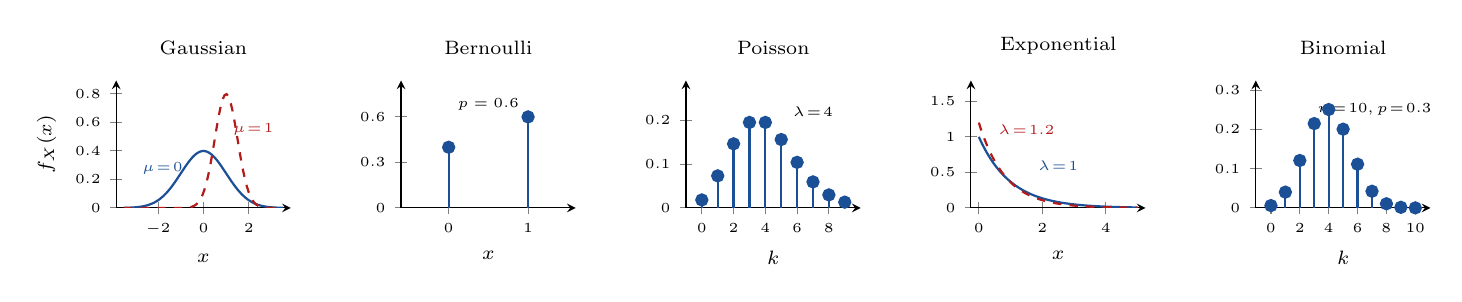
\begin{tikzpicture}
\begin{groupplot}[
  group style={
    group size=5 by 1,
    horizontal sep=1.4cm,
    vertical sep=0cm,
  },
  width=3.8cm, height=3.2cm,
  axis lines=left,
  tick style={thin,black!50},
  tick label style={font=\tiny},
  label style={font=\scriptsize},
  ymin=0,
  enlarge x limits=0.05,
  enlarge y limits={upper,value=0.12},
  grid=none,
]

% Gaussian
\nextgroupplot[title={\scriptsize Gaussian},xlabel={$x$},ylabel={$f_X(x)$},
  domain=-3.5:3.5, samples=80]
\addplot[thick,tufteblue] {exp(-x^2/2)/sqrt(2*pi)};
\addplot[thick,tuftered,dashed,domain=-3.5:3.5,samples=80] {exp(-(x-1)^2/(2*0.5^2))/(sqrt(2*pi)*0.5)};
\node[font=\tiny,tufteblue] at (axis cs:-1.8,0.28) {$\mu\!=\!0$};
\node[font=\tiny,tuftered] at (axis cs:2.2,0.55) {$\mu\!=\!1$};

% Bernoulli
\nextgroupplot[title={\scriptsize Bernoulli},xlabel={$x$},
  xtick={0,1},xmin=-0.5,xmax=1.5,ytick={0,0.3,0.6},ymax=0.75]
\addplot+[ycomb,thick,tufteblue,mark=*,mark options={fill=tufteblue}]
  coordinates {(0,0.4)(1,0.6)};
\node[font=\tiny] at (axis cs:0.5,0.68) {$p=0.6$};

% Poisson
\nextgroupplot[title={\scriptsize Poisson},xlabel={$k$},
  xmin=-0.5,xmax=9.5,xtick={0,2,4,6,8},ymax=0.26]
\addplot+[ycomb,thick,tufteblue,mark=*,mark options={fill=tufteblue}]
  coordinates {(0,0.0183)(1,0.0733)(2,0.1465)(3,0.1954)(4,0.1954)
               (5,0.1563)(6,0.1042)(7,0.0595)(8,0.0298)(9,0.0132)};
\node[font=\tiny] at (axis cs:7,0.22) {$\lambda\!=\!4$};

% Exponential
\nextgroupplot[title={\scriptsize Exponential},xlabel={$x$},
  domain=0:5,samples=80,xmin=0,xmax=5,ymax=1.6]
\addplot[thick,tufteblue] {exp(-x)};
\addplot[thick,tuftered,dashed] {1.2*exp(-1.2*x)};
\node[font=\tiny,tufteblue] at (axis cs:2.5,0.6) {$\lambda\!=\!1$};
\node[font=\tiny,tuftered] at (axis cs:1.5,1.1) {$\lambda\!=\!1.2$};

% Binomial
\nextgroupplot[title={\scriptsize Binomial},xlabel={$k$},
  xmin=-0.5,xmax=10.5,xtick={0,2,4,6,8,10},ymax=0.29]
\addplot+[ycomb,thick,tufteblue,mark=*,mark options={fill=tufteblue}]
  coordinates {(0,0.0060)(1,0.0403)(2,0.1209)(3,0.2150)(4,0.2508)
               (5,0.2007)(6,0.1115)(7,0.0425)(8,0.0106)(9,0.0016)(10,0.0001)};
\node[font=\tiny] at (axis cs:7.5,0.25) {$n\!=\!10,p\!=\!0.35$};

\end{groupplot}
\end{tikzpicture}
\caption{The five distributions introduced in this section. \textit{Blue}: primary parameter choice; \textit{dashed red}: alternative parameter.}
\label{fig:distributions}
\end{figure*}

\subsection{Classic distributions}

\newthought{The five distributions} shown in Figure~\ref{fig:distributions} appear throughout the course.

\medskip
\noindent\textbf{Gaussian.}\quad $X\sim\N(\mu,\sigma^2)$ has pdf
\begin{equation}
  f_X(x)=\frac{1}{\sqrt{2\pi\sigma^2}}\exp\!\left(-\frac{(x-\mu)^2}{2\sigma^2}\right), \quad x\in\mathbb{R}.
  \label{eq:gaussian_pdf}
\end{equation}
It maximises entropy subject to fixed mean and variance, and is the attractor for sums of finite-variance variables (CLT).

\medskip
\noindent\textbf{Bernoulli.}\quad $X\sim\text{Bernoulli}(p)$: $P(X=x)=p^x(1-p)^{1-x}$, $x\in\{0,1\}$.
Mean $p$, variance $p(1-p)$.

\medskip
\noindent\textbf{Binomial.}\quad $X\sim\text{Binomial}(n,p)$: $P(X=k)=\binom{n}{k}p^k(1-p)^{n-k}$.
Mean $np$, variance $np(1-p)$.

\medskip
\noindent\textbf{Poisson.}\quad $X\sim\text{Poisson}(\lambda)$: $P(X=k)=e^{-\lambda}\lambda^k/k!$.
Mean $=$ variance $=\lambda$.

\medskip
\noindent\textbf{Exponential.}\quad $X\sim\text{Exp}(\lambda)$: $f_X(x)=\lambda e^{-\lambda x}$, $x\geq 0$.
The only continuous memoryless distribution.

% ============================================================
\section{Generating functions}
% ============================================================

\newthought{Three generating functions} encode all statistical information in a distribution. They are the main calculational tools we will use to manipulate and identify distributions.

\subsection{Moment generating function}

The \textbf{moment generating function} (MGF) is
\begin{equation}
  M_X(t)=\E[e^{tX}]=\int_{-\infty}^{\infty} e^{tx}f_X(x)\,\d x.
  \label{eq:mgf_def}
\end{equation}
Expanding $e^{tX}=\sum_{n=0}^\infty (tX)^n/n!$ and taking expectations term by term,
\begin{equation}
  M_X(t)=\sum_{n=0}^\infty \frac{t^n}{n!}\E[X^n],
\end{equation}
so the $n$-th moment is recovered by differentiation:
\begin{keyresult}
\begin{equation}
  \E[X^n]=\left.\frac{\d^n M_X}{\d t^n}\right|_{t=0}.
  \label{eq:moment_from_MGF}
\end{equation}
\end{keyresult}
For independent $X,Y$, the MGF of the sum factorises:
$M_{X+Y}(t)=M_X(t)M_Y(t)$,
since $\E[e^{t(X+Y)}]=\E[e^{tX}]\E[e^{tY}]$ under independence.

\noindent\textit{\textbf{MGF of the Gaussian}}\quad

For $X\sim\N(\mu,\sigma^2)$:
\begin{equation}
  M_X(t)=\int_{-\infty}^{\infty} e^{tx}\,\frac{1}{\sqrt{2\pi\sigma^2}}\exp\!\left(-\frac{(x-\mu)^2}{2\sigma^2}\right)\d x.
\end{equation}
Combine the exponentials:
\begin{equation}
  tx-\frac{(x-\mu)^2}{2\sigma^2}
  =-\frac{(x-(\mu+\sigma^2 t))^2}{2\sigma^2}+\mu t+\frac{\sigma^2 t^2}{2}.
\end{equation}
The constant terms factor out; the remaining integral is a Gaussian normalisation equal to 1:
\begin{keyresult}
\begin{equation}
  M_X(t)=\exp\!\left(\mu t+\tfrac{1}{2}\sigma^2 t^2\right).
  \label{eq:gaussian_mgf}
\end{equation}
\end{keyresult}
Differentiating at $t=0$ gives $\E[X]=\mu$ and $\var(X)=\sigma^2$.

\noindent\textit{\textbf{MGF of the Bernoulli}}\quad

$M_X(t)=(1-p)+pe^t$. Then $M_X'(0)=p$ and $\var(X)=M_X''(0)-(M_X'(0))^2=p(1-p)$.

\subsection{Cumulant generating function}

The \textbf{cumulant generating function} (CGF) is
\begin{equation}
  K_X(t)=\log M_X(t),
  \label{eq:cgf_def}
\end{equation}
and the $n$-th \textbf{cumulant} is $\kappa_n=K_X^{(n)}(0)$. The first two are $\kappa_1=\E[X]$ and $\kappa_2=\var(X)$; higher cumulants measure non-Gaussianity ($\kappa_3$ is skewness, $\kappa_4$ is excess kurtosis). All cumulants of a Gaussian beyond the second vanish.

\newthought{Why the logarithm?} Because for independent $X,Y$,
\begin{equation}
  K_{X+Y}(t)=K_X(t)+K_Y(t).
\end{equation}
Cumulants are additive for independent variables; moments are not. This makes the CGF the natural tool for large-system analysis.

\noindent\textit{\textbf{CGF of the Gaussian}}\quad

$K_X(t)=\mu t+\frac{1}{2}\sigma^2 t^2$. The CGF is a polynomial of degree 2 — the hallmark of the Gaussian. Hence $\kappa_1=\mu$, $\kappa_2=\sigma^2$, $\kappa_n=0$ for $n\geq 3$.

\noindent\textit{\textbf{CGF of the Poisson}}\quad

The MGF is $M_X(t)=e^{-\lambda}\sum_k(\lambda e^t)^k/k!=\exp(\lambda(e^t-1))$, so
\begin{equation}
  K_X(t)=\lambda(e^t-1), \qquad \kappa_n=\lambda\;\;\forall n\geq 1.
\end{equation}
All cumulants equal $\lambda$, confirming $\E[X]=\var(X)=\lambda$.

\subsection{Characteristic function}

The \textbf{characteristic function} (Fourier transform of $f_X$) is
\begin{equation}
  \phi_X(t)=\E[e^{itX}]=\int_{-\infty}^{\infty} e^{itx}f_X(x)\,\d x, \quad t\in\mathbb{R}.
  \label{eq:cf_def}
\end{equation}
It always exists since $|e^{itx}|=1$, and it \emph{uniquely} determines the distribution even when the MGF does not exist (heavy tails). The inversion formula reconstructs the pdf:
\begin{equation}
  f_X(x)=\frac{1}{2\pi}\int_{-\infty}^{\infty} e^{-itx}\phi_X(t)\,\d t.
  \label{eq:cf_inversion}
\end{equation}

\noindent\textbf{Gaussian.}\quad $\phi_X(t)=\exp(i\mu t-\frac{1}{2}\sigma^2 t^2)$, obtained by substituting $t\to it$ in~\eqref{eq:gaussian_mgf}.

\medskip
Figure~\ref{fig:gen_functions} summarises the relationships among the three generating functions.

\begin{figure}
\centering
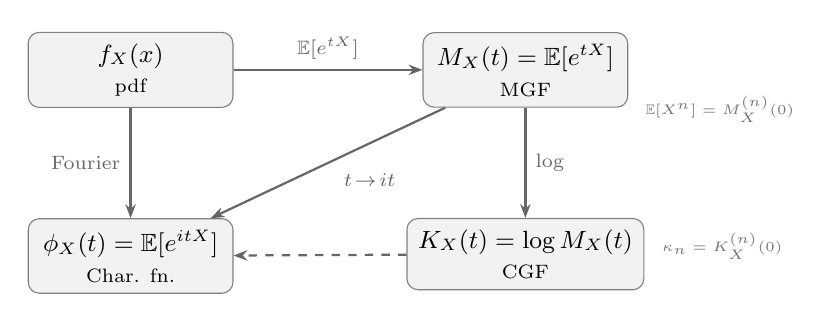
\begin{tikzpicture}[
  node distance=1.5cm and 2.4cm,
  box/.style={draw=black!50, fill=black!5, rounded corners=4pt,
              minimum width=2.6cm, minimum height=0.85cm,
              font=\small, align=center, inner sep=4pt},
  arr/.style={-{Stealth[length=5pt]}, thick, black!60},
  label/.style={font=\scriptsize, midway}
]
\node[box] (pdf) {$f_X(x)$ \\ \scriptsize pdf};
\node[box, right=of pdf] (mgf) {$M_X(t)=\E[e^{tX}]$ \\ \scriptsize MGF};
\node[box, below=1.4cm of mgf] (cgf) {$K_X(t)=\log M_X(t)$ \\ \scriptsize CGF};
\node[box, below=1.4cm of pdf] (cf)  {$\phi_X(t)=\E[e^{itX}]$ \\ \scriptsize Char. fn.};

\draw[arr] (pdf) -- node[label,above]{$\E[e^{tX}]$} (mgf);
\draw[arr] (pdf) -- node[label,left]{Fourier} (cf);
\draw[arr] (mgf) -- node[label,right]{$\log$} (cgf);
\draw[arr] (mgf) -- node[label,below right,xshift=2pt]{$t\!\to\! it$} (cf);
\draw[arr,dashed] (cgf) -- node[label,below]{} (cf);

% annotations
\node[font=\tiny, text=black!55, right=0.1cm of mgf, yshift=-0.5cm]
  {$\E[X^n]=M^{(n)}_X(0)$};
\node[font=\tiny, text=black!55, right=0.1cm of cgf, yshift=0.1cm]
  {$\kappa_n=K^{(n)}_X(0)$};
\end{tikzpicture}
\caption{Relationships among the three generating functions. Arrows show how each is constructed from the previous.}
\label{fig:gen_functions}
\end{figure}

% ============================================================
\section{Multivariate distributions}
% ============================================================

\newthought{For two random variables} $X,Y$ the \textbf{joint pdf} $f_{X,Y}(x,y)$ satisfies $\iint f_{X,Y}\,\d x\,\d y=1$. The \textbf{marginal} pdfs are
\begin{equation}
  f_X(x)=\int f_{X,Y}(x,y)\,\d y, \qquad f_Y(y)=\int f_{X,Y}(x,y)\,\d x.
\end{equation}
The \textbf{conditional} pdf is $f_{X|Y}(x|y)=f_{X,Y}(x,y)/f_Y(y)$, which is Bayes' theorem in density form: $f_{X|Y}(x|y)\propto f_{Y|X}(y|x)\,f_X(x)$.

$X$ and $Y$ are \textbf{independent} iff $f_{X,Y}=f_X f_Y$. The \textbf{covariance} and \textbf{correlation} are
\begin{equation}
  \mathrm{Cov}(X,Y)=\E[XY]-\E[X]\E[Y], \qquad
  \rho=\frac{\mathrm{Cov}(X,Y)}{\sqrt{\var(X)\var(Y)}}\in[-1,1].
\end{equation}

\subsection{The multivariate Gaussian}

A random vector $\vec{x}\in\mathbb{R}^N$ follows $\vec{x}\sim\N(\boldsymbol{\mu},\mathbf{C})$ if
\begin{keyresult}
\begin{equation}
  f(\vec{x})=\frac{1}{\sqrt{(2\pi)^N\det\mathbf{C}}}\exp\!\left(-\tfrac{1}{2}(\vec{x}-\boldsymbol{\mu})^T\mathbf{C}^{-1}(\vec{x}-\boldsymbol{\mu})\right).
  \label{eq:multivariate_gaussian}
\end{equation}
\end{keyresult}
We derive this form from first principles in Section~\ref{sec:gaussian_integrals}.

% ============================================================
\section{Gaussian integrals}
\label{sec:gaussian_integrals}
% ============================================================

\newthought{Gaussian integrals} are the fundamental computational engine of statistical physics and machine learning theory. The ability to evaluate them in closed form — even in hundreds of dimensions — is what makes Gaussian models analytically tractable.

\subsection{The one-dimensional integral}

\begin{keyresult}
\begin{equation}
  \int_{-\infty}^{\infty} e^{-\frac{1}{2}ax^2}\,\d x = \sqrt{\frac{2\pi}{a}}, \quad a>0.
  \label{eq:gauss_1d}
\end{equation}
\end{keyresult}

\noindent\textbf{Derivation.} Let $I=\int e^{-\frac{a}{2}x^2}\d x$ and square it:
\begin{equation}
  I^2=\iint e^{-\frac{a}{2}(x^2+y^2)}\d x\,\d y.
\end{equation}
Switch to polar coordinates $x=r\cos\theta$, $y=r\sin\theta$, with area element $r\,\d r\,\d\theta$:
\begin{equation}
  I^2=2\pi\int_0^\infty r\,e^{-\frac{a}{2}r^2}\d r.
\end{equation}
Substitute $u=\frac{a}{2}r^2$ so $r\,\d r=\d u/a$:
\begin{equation}
  I^2=\frac{2\pi}{a}\int_0^\infty e^{-u}\d u=\frac{2\pi}{a},
\end{equation}
giving $I=\sqrt{2\pi/a}$. The polar-coordinates trick is illustrated in the margin.

\begin{marginfigure}
\centering
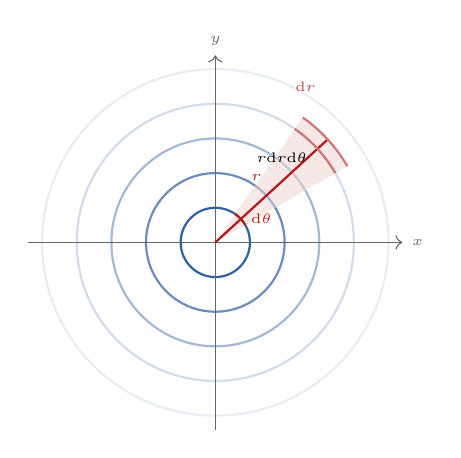
\begin{tikzpicture}[scale=0.88]
% contour rings of the 2d Gaussian
\foreach \r/\op in {0.5/0.9,1.0/0.65,1.5/0.40,2.0/0.20,2.5/0.10}{
  \draw[tufteblue,opacity=\op,thick] (0,0) circle (\r);
}
% axes
\draw[->,thin,black!60] (-2.7,0)--(2.7,0) node[right,font=\tiny]{$x$};
\draw[->,thin,black!60] (0,-2.7)--(0,2.7) node[above,font=\tiny]{$y$};
% polar wedge
\fill[tuftered!20,opacity=0.5]
  (0,0) -- ({2.2*cos(30)},{2.2*sin(30)}) arc (30:55:2.2) -- cycle;
\draw[tuftered,thick] (0,0) -- ({2.2*cos(42.5)},{2.2*sin(42.5)})
  node[midway,above left,font=\tiny,tuftered]{$r$};
\draw[tuftered,thick] ({0.5*cos(30)},{0.5*sin(30)}) arc (30:55:0.5)
  node[midway,right,font=\tiny,tuftered]{$\d\theta$};
% dr arc
\draw[tuftered!60,thick]
  ({2.0*cos(30)},{2.0*sin(30)}) arc (30:55:2.0);
\draw[tuftered!60,thick]
  ({2.2*cos(30)},{2.2*sin(30)}) arc (30:55:2.2);
\node[font=\tiny,tuftered!80] at ({2.6*cos(60)},{2.6*sin(60)}){$\d r$};
% area label
\node[font=\tiny] at ({1.3*cos(42.5)},{1.3*sin(42.5)+0.35}){$r\d r\d\theta$};
\end{tikzpicture}
\caption{Squaring $I$ converts the product of two 1-D Gaussians into a 2-D radially symmetric integral. The area element in polar coordinates is $r\,\d r\,\d\theta$.}
\label{fig:polar_gaussian}
\end{marginfigure}

Adding a linear source term by completing the square,
$-\frac{a}{2}x^2+bx=-\frac{a}{2}(x-b/a)^2+b^2/(2a)$,
and shifting $x\to x+b/a$:
\begin{keyresult}
\begin{equation}
  \int_{-\infty}^{\infty} e^{-\frac{1}{2}ax^2+bx}\,\d x = \sqrt{\frac{2\pi}{a}}\,e^{\frac{b^2}{2a}}.
  \label{eq:gauss_1d_source}
\end{equation}
\end{keyresult}

\subsection{The multidimensional integral}

Let $\vec{x}\in\mathbb{R}^N$, $\mathbf{A}$ real symmetric positive-definite, $\vec{b}\in\mathbb{R}^N$. Then:
\begin{keyresult}
\begin{equation}
  \int_{\mathbb{R}^N}\!\d^N\!x\;\exp\!\left(-\tfrac{1}{2}\vec{x}^T\mathbf{A}\vec{x}+\vec{b}^T\vec{x}\right)
  =\sqrt{\frac{(2\pi)^N}{\det\mathbf{A}}}\;\exp\!\left(\tfrac{1}{2}\vec{b}^T\mathbf{A}^{-1}\vec{b}\right).
  \label{eq:gauss_Nd}
\end{equation}
\end{keyresult}

\textbf{Step 1: Complete the square.} Claim:
\begin{equation}
  -\tfrac{1}{2}\vec{x}^T\mathbf{A}\vec{x}+\vec{b}^T\vec{x}
  =-\tfrac{1}{2}(\vec{x}-\mathbf{A}^{-1}\vec{b})^T\mathbf{A}(\vec{x}-\mathbf{A}^{-1}\vec{b})
   +\tfrac{1}{2}\vec{b}^T\mathbf{A}^{-1}\vec{b}.
  \label{eq:complete_square}
\end{equation}
Expanding the right-hand side and using $\mathbf{A}\mathbf{A}^{-1}=\mathbf{I}$ and symmetry of $\mathbf{A}$:
\begin{align}
  \text{RHS}
  &=-\tfrac{1}{2}\vec{x}^T\mathbf{A}\vec{x}
    +\tfrac{1}{2}\vec{x}^T\vec{b}
    +\tfrac{1}{2}\vec{b}^T\vec{x}\nonumber\\
  &\quad
    -\tfrac{1}{2}\vec{b}^T\mathbf{A}^{-1}\vec{b}
    +\tfrac{1}{2}\vec{b}^T\mathbf{A}^{-1}\vec{b}\nonumber\\
  &=-\tfrac{1}{2}\vec{x}^T\mathbf{A}\vec{x}+\vec{b}^T\vec{x},
\end{align}
confirming~\eqref{eq:complete_square}.

\textbf{Step 2: Shift the variable.} Set $\vec{y}=\vec{x}-\mathbf{A}^{-1}\vec{b}$ ($\d^N y=\d^N x$):
\begin{equation}
  \int\d^N\!x\;e^{-\frac{1}{2}\vec{x}^T\mathbf{A}\vec{x}+\vec{b}^T\vec{x}}
  =e^{\frac{1}{2}\vec{b}^T\mathbf{A}^{-1}\vec{b}}\int\d^N\!y\;e^{-\frac{1}{2}\vec{y}^T\mathbf{A}\vec{y}}.
  \label{eq:shift_int}
\end{equation}

\textbf{Step 3: Diagonalise $\mathbf{A}$.} By the spectral theorem $\mathbf{A}=\mathbf{O}^T\boldsymbol{\Lambda}\mathbf{O}$ with $\mathbf{O}$ orthogonal and $\boldsymbol{\Lambda}=\mathrm{diag}(\lambda_1,\ldots,\lambda_N)$, $\lambda_i>0$. Set $\vec{u}=\mathbf{O}\vec{y}$, so $\d^N u=\d^N y$ and $\vec{y}^T\mathbf{A}\vec{y}=\sum_i\lambda_i u_i^2$. The integral factorises:
\begin{equation}
  \int\d^N\!y\;e^{-\frac{1}{2}\vec{y}^T\mathbf{A}\vec{y}}
  =\prod_{i=1}^N\sqrt{\frac{2\pi}{\lambda_i}}
  =\sqrt{\frac{(2\pi)^N}{\det\mathbf{A}}}.
  \label{eq:diagonal_int}
\end{equation}
Combining~\eqref{eq:shift_int} and~\eqref{eq:diagonal_int} gives~\eqref{eq:gauss_Nd}.

\begin{figure*}[t]
\centering
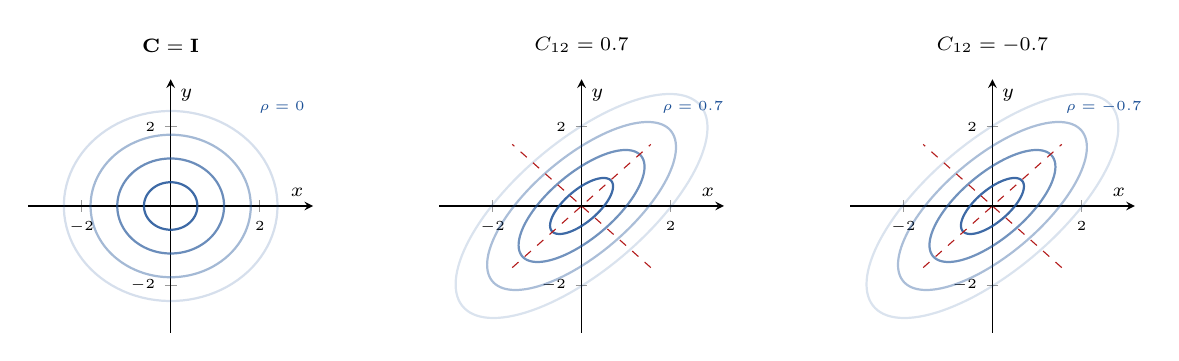
\begin{tikzpicture}
\begin{groupplot}[
  group style={group size=3 by 1, horizontal sep=1.6cm},
  width=5.2cm, height=4.8cm,
  axis lines=center,
  tick style={thin,black!40},
  tick label style={font=\tiny},
  label style={font=\scriptsize},
  xlabel={$x$}, ylabel={$y$},
  xmin=-3.2,xmax=3.2, ymin=-3.2,ymax=3.2,
  grid=none,
  clip=false,
]

% --- Isotropic Gaussian: C = I ---
\nextgroupplot[title={\scriptsize $\mathbf{C}=\mathbf{I}$}]
\addplot[tufteblue,thick,opacity=0.85,domain=0:360,samples=100] ({0.6*cos(x)},{0.6*sin(x)});
\addplot[tufteblue,thick,opacity=0.65,domain=0:360,samples=100] ({1.2*cos(x)},{1.2*sin(x)});
\addplot[tufteblue,thick,opacity=0.40,domain=0:360,samples=100] ({1.8*cos(x)},{1.8*sin(x)});
\addplot[tufteblue,thick,opacity=0.18,domain=0:360,samples=100] ({2.4*cos(x)},{2.4*sin(x)});
\node[font=\tiny,tufteblue] at (2.5,2.5) {$\rho=0$};

% --- Correlated Gaussian: C = [[1,0.7],[0.7,1]] ---
% eigenvalues 1.7 and 0.3; eigenvectors (1,1)/sqrt2 and (1,-1)/sqrt2
\nextgroupplot[title={\scriptsize $C_{12}=0.7$}]
\addplot[tufteblue,thick,opacity=0.85,domain=0:360,samples=120]
  ({(0.5*1.304*cos(x)+0.5*0.548*sin(x))},{(0.5*1.304*cos(x)-0.5*0.548*sin(x))});
\addplot[tufteblue,thick,opacity=0.62,domain=0:360,samples=120]
  ({(1.0*1.304*cos(x)+1.0*0.548*sin(x))},{(1.0*1.304*cos(x)-1.0*0.548*sin(x))});
\addplot[tufteblue,thick,opacity=0.37,domain=0:360,samples=120]
  ({(1.5*1.304*cos(x)+1.5*0.548*sin(x))},{(1.5*1.304*cos(x)-1.5*0.548*sin(x))});
\addplot[tufteblue,thick,opacity=0.16,domain=0:360,samples=120]
  ({(2.0*1.304*cos(x)+2.0*0.548*sin(x))},{(2.0*1.304*cos(x)-2.0*0.548*sin(x))});
\node[font=\tiny,tufteblue] at (2.5,2.5) {$\rho=0.7$};
% principal axes
\draw[tuftered,thin,dashed] ({-1.556},{-1.556}) -- ({1.556},{1.556});
\draw[tuftered,thin,dashed] ({1.556},{-1.556}) -- ({-1.556},{1.556});

% --- Negatively correlated: C = [[1,-0.7],[-0.7,1]] ---
\nextgroupplot[title={\scriptsize $C_{12}=-0.7$}]
\addplot[tufteblue,thick,opacity=0.85,domain=0:360,samples=120]
  ({(0.5*1.304*cos(x)-0.5*0.548*sin(x))},{(0.5*1.304*cos(x)+0.5*0.548*sin(x))});
\addplot[tufteblue,thick,opacity=0.62,domain=0:360,samples=120]
  ({(1.0*1.304*cos(x)-1.0*0.548*sin(x))},{(1.0*1.304*cos(x)+1.0*0.548*sin(x))});
\addplot[tufteblue,thick,opacity=0.37,domain=0:360,samples=120]
  ({(1.5*1.304*cos(x)-1.5*0.548*sin(x))},{(1.5*1.304*cos(x)+1.5*0.548*sin(x))});
\addplot[tufteblue,thick,opacity=0.16,domain=0:360,samples=120]
  ({(2.0*1.304*cos(x)-2.0*0.548*sin(x))},{(2.0*1.304*cos(x)+2.0*0.548*sin(x))});
\node[font=\tiny,tufteblue] at (2.5,2.5) {$\rho=-0.7$};
\draw[tuftered,thin,dashed] ({1.556},{-1.556}) -- ({-1.556},{1.556});
\draw[tuftered,thin,dashed] ({-1.556},{-1.556}) -- ({1.556},{1.556});

\end{groupplot}
\end{tikzpicture}
\caption{Level sets (constant-density contours) of 2-D Gaussians. Left: isotropic ($\mathbf{C}=\mathbf{I}$), circular contours. Centre: positive correlation $\rho=0.7$, ellipse tilted at $45°$. Right: negative correlation $\rho=-0.7$, ellipse tilted at $-45°$. Dashed red lines mark the principal axes (eigenvectors of $\mathbf{C}$).}
\label{fig:2d_gaussian}
\end{figure*}

\subsection{The source trick and moment generation}

Define the \textbf{generating functional}\sidenote{The name \emph{generating functional} comes from field theory; here it is simply the Gaussian integral as a function of the source $\vec{b}$.}
\begin{equation}
  Z(\vec{b})=\int\d^N\!x\; e^{-\frac{1}{2}\vec{x}^T\mathbf{A}\vec{x}+\vec{b}^T\vec{x}}
  =Z_0\,e^{\frac{1}{2}\vec{b}^T\mathbf{A}^{-1}\vec{b}},
  \label{eq:generating_functional}
\end{equation}
where $Z_0=Z(\vec{0})=\sqrt{(2\pi)^N/\det\mathbf{A}}$. Since $\partial e^{\vec{b}^T\vec{x}}/\partial b_i=x_i e^{\vec{b}^T\vec{x}}$, differentiating and setting $\vec{b}=\vec{0}$ extracts moments:
\begin{equation}
  \langle x_i\rangle=\frac{1}{Z_0}\frac{\partial Z}{\partial b_i}\bigg|_{\vec{b}=\vec{0}}.
\end{equation}

\textbf{First moment.}
$\partial Z/\partial b_i = Z(\vec{b})(\mathbf{A}^{-1}\vec{b})_i$.
At $\vec{b}=\vec{0}$: $\langle x_i\rangle=0$.

\textbf{Second moment.} Differentiating again:
\begin{align}
  \frac{\partial^2 Z}{\partial b_i\partial b_j}\bigg|_{\vec{b}=\vec{0}}
  &=Z_0(\mathbf{A}^{-1})_{ij},
\end{align}
so
\begin{keyresult}
\begin{equation}
  \langle x_i x_j\rangle=(\mathbf{A}^{-1})_{ij}=C_{ij}.
  \label{eq:propagator}
\end{equation}
\end{keyresult}
\emph{The two-point correlator equals the $(i,j)$ entry of the inverse of the matrix in the exponent.} We call $C_{ij}$ the \textbf{propagator}. The level sets of 2-D Gaussians for different covariance structures are shown in Figure~\ref{fig:2d_gaussian}.

% ============================================================
\section{Wick's theorem}
\label{sec:wicks_theorem}
% ============================================================

\newthought{Wick's theorem} gives an algorithmic rule for computing any moment of a Gaussian in terms of the propagator alone. It is the central combinatorial identity of perturbative field theory.

\subsection{Statement}

Let $\vec{x}\sim\N(\vec{0},\mathbf{C})$. Then:
\begin{enumerate}[leftmargin=*,label=(\arabic*)]
  \item All odd moments vanish.
  \item All even moments satisfy:
\begin{keyresult}
\begin{equation}
  \langle x_{i_1}x_{i_2}\cdots x_{i_{2n}}\rangle
  =\sum_{\text{pairings}}\prod_{\text{pairs }(j,k)} C_{i_j i_k},
  \label{eq:wicks_theorem}
\end{equation}
\end{keyresult}
where the sum runs over all $(2n-1)!!=1\cdot 3\cdot 5\cdots(2n-1)$ distinct ways to pair $\{i_1,\ldots,i_{2n}\}$ into $n$ unordered pairs.
\end{enumerate}

\subsection{Derivation via the generating functional}

With $Z(\vec{b})=Z_0 e^{\frac{1}{2}\vec{b}^T\mathbf{C}\vec{b}}$, expand:
\begin{equation}
  e^{\frac{1}{2}\vec{b}^T\mathbf{C}\vec{b}}=\sum_{n=0}^\infty\frac{1}{n!}\left(\frac{1}{2}\sum_{i,j}b_i C_{ij}b_j\right)^n.
  \label{eq:Z_expansion}
\end{equation}
The $m$-th moment is $\langle x_{i_1}\cdots x_{i_m}\rangle=\partial^m e^{\frac{1}{2}\vec{b}^T\mathbf{C}\vec{b}}/\partial b_{i_1}\cdots\partial b_{i_m}|_{\vec{b}=\vec{0}}$.

For odd $m=2n+1$: every term in~\eqref{eq:Z_expansion} has even powers of $\vec{b}$; after $2n+1$ derivatives at least one $b$ factor remains, which vanishes at $\vec{0}$. All odd moments vanish.

For even $m=2n$: only the $n$-th term in~\eqref{eq:Z_expansion} survives. Expanding it,
\begin{equation}
  \frac{1}{n!2^n}\sum_{i_1,j_1}\cdots\sum_{i_n,j_n} C_{i_1 j_1}\cdots C_{i_n j_n}\;b_{i_1}b_{j_1}\cdots b_{i_n}b_{j_n}.
\end{equation}
Differentiating $2n$ times matches each $b_{k_l}$ to exactly one index; the $\frac{1}{n!\,2^n}$ prefactor precisely cancels the $n!\,2^n$ over-counting of pairings, leaving the sum over distinct pairings of products of $C_{k_a k_b}$. This is Eq.~\eqref{eq:wicks_theorem}.

\subsection{Worked examples}

\noindent\textit{\textbf{Fourth moment}}\quad

For $X\sim\N(0,\sigma^2)$ there are $(4-1)!!=3$ pairings of $\{1,2,3,4\}$:

\begin{marginfigure}
\centering
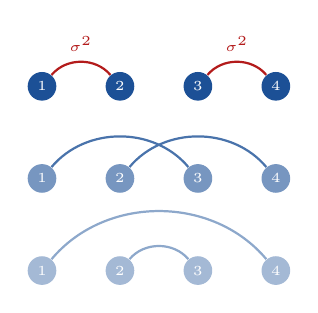
\begin{tikzpicture}[scale=0.9]
% three Wick pairings visualised as arcs
\def\pts{4}
\foreach \i in {1,...,4}{
  \node[circle,fill=tufteblue,inner sep=2pt,font=\tiny\color{white}]
    (v\i) at ({(\i-1)*1.1},0) {\i};
}
% Pairing 1: (12)(34) — top arcs
\draw[tuftered,thick] (v1) to[bend left=50] node[above,font=\tiny]{$\sigma^2$} (v2);
\draw[tuftered,thick] (v3) to[bend left=50] node[above,font=\tiny]{$\sigma^2$} (v4);
% Pairing 2: (13)(24)
\begin{scope}[yshift=-1.3cm]
\foreach \i in {1,...,4}{
  \node[circle,fill=tufteblue!60,inner sep=2pt,font=\tiny\color{white}]
    (w\i) at ({(\i-1)*1.1},0) {\i};
}
\draw[tufteblue!80,thick] (w1) to[bend left=50] (w3);
\draw[tufteblue!80,thick] (w2) to[bend left=50] (w4);
\end{scope}
% Pairing 3: (14)(23)
\begin{scope}[yshift=-2.6cm]
\foreach \i in {1,...,4}{
  \node[circle,fill=tufteblue!40,inner sep=2pt,font=\tiny\color{white}]
    (u\i) at ({(\i-1)*1.1},0) {\i};
}
\draw[tufteblue!50,thick] (u1) to[bend left=50] (u4);
\draw[tufteblue!50,thick] (u2) to[bend left=50] (u3);
\end{scope}
\end{tikzpicture}
\caption{The three Wick pairings of $\{1,2,3,4\}$ for computing $\langle X^4\rangle$. Each arc contributes a propagator $\sigma^2$.}
\label{fig:wick_pairings}
\end{marginfigure}

\begin{itemize}[leftmargin=*]
  \item $(1,2)(3,4)$: contributes $\sigma^2\cdot\sigma^2=\sigma^4$.
  \item $(1,3)(2,4)$: contributes $\sigma^4$.
  \item $(1,4)(2,3)$: contributes $\sigma^4$.
\end{itemize}
So $\langle X^4\rangle=3\sigma^4$. (The three pairings are illustrated in the margin.) Verification via the MGF: differentiating $e^{\frac{1}{2}\sigma^2 t^2}$ four times at $t=0$ gives $3\sigma^4$. $\checkmark$

\noindent\textit{\textbf{Two-variable moment}}\quad

For $(x_1,x_2)\sim\N(\vec{0},\mathbf{C})$, the three pairings of $(1,1,2,2)$ give
\begin{equation}
  \langle x_1^2 x_2^2\rangle=C_{11}C_{22}+2C_{12}^2.
\end{equation}
For independent variables ($C_{12}=0$) this reduces to $\langle x_1^2\rangle\langle x_2^2\rangle$. $\checkmark$

\noindent\textit{\textbf{Sixth moment}}\quad

$(6-1)!!=15$ pairings, each contributing $\sigma^6$, so $\langle X^6\rangle=15\sigma^6$.

% ============================================================
\section{Saddle-point approximation}
\label{sec:saddle_point}
% ============================================================

\newthought{Many integrals} in statistical physics and machine learning take the form
\begin{equation}
  I(N)=\int_{-\infty}^{\infty}\d x\; e^{-Nf(x)},
  \label{eq:laplace_integral}
\end{equation}
where $N$ is a large parameter (number of neurons, spins, data points) and $f(x)$ is smooth. As $N\to\infty$, the integrand concentrates exponentially near the minimum of $f$.

\subsection{One-dimensional case}

Let $x^*$ minimise $f$: $f'(x^*)=0$, $f''(x^*)>0$. Taylor expand:
\begin{equation}
  f(x)=f(x^*)+\underbrace{f'(x^*)}_{0}(x-x^*)+\frac{f''(x^*)}{2}(x-x^*)^2+\cdots
\end{equation}
Substituting and evaluating the Gaussian integral:
\begin{keyresult}
\begin{equation}
  I(N)\approx\sqrt{\frac{2\pi}{Nf''(x^*)}}\,e^{-Nf(x^*)}, \qquad N\to\infty.
  \label{eq:saddle_point_1d}
\end{equation}
\end{keyresult}
The cubic correction is $\mathcal{O}(N^{-1/2})\to 0$ since fluctuations are of order $(x-x^*)\sim N^{-1/2}$.

\begin{marginfigure}
\centering
\begin{tikzpicture}
\begin{axis}[
  tufte axis,
  width=\linewidth, height=0.9\linewidth,
  xlabel={$x$},
  ylabel={},
  xmin=-0.5, xmax=2.5,
  ymin=-0.05, ymax=1.1,
  xtick={1},
  xticklabels={$x^*$},
  ytick=\empty,
  title={\scriptsize Saddle-point concentration},
  axis lines=left,
]
% f(x) = (x-1)^2 + 0.3 (x-1)^4
\addplot[black!70, thick, domain=0.05:2.3, samples=80]
  {(0.35*(x-1)^2 + 0.06*(x-1)^4 + 0.05};
% N=5 integrand
\addplot[tufteblue, thick, domain=0.2:1.8, samples=80]
  {exp(-5*(0.35*(x-1)^2))};
% N=20 integrand
\addplot[tuftered, thick, domain=0.6:1.4, samples=80]
  {exp(-20*(0.35*(x-1)^2))};
\node[font=\tiny,tufteblue] at (axis cs:0.35,0.55){$N=5$};
\node[font=\tiny,tuftered] at (axis cs:0.72,0.82){$N=20$};
\node[font=\tiny,black!60] at (axis cs:2.1,0.65){$f(x)$};
% vertical dashed line at saddle
\addplot[black!30,dashed,thin] coordinates {(1,0)(1,1)};
\end{axis}
\end{tikzpicture}
\caption{As $N$ grows, $e^{-Nf(x)}$ concentrates ever more sharply near $x^*$. The saddle-point approximation replaces $f$ with its quadratic expansion around $x^*$.}
\label{fig:saddle_point}
\end{marginfigure}

\subsection{Multidimensional case}

For $\vec{x}^*$ with $\nabla f(\vec{x}^*)=\vec{0}$ and Hessian $\mathbf{H}_{ij}=\partial^2 f/\partial x_i\partial x_j|_{\vec{x}^*}$:
\begin{keyresult}
\begin{equation}
  \int_{\mathbb{R}^N}\d^N\!x\;e^{-Nf(\vec{x})}
  \approx\left(\frac{2\pi}{N}\right)^{N/2}\frac{e^{-Nf(\vec{x}^*)}}{\sqrt{\det\mathbf{H}(\vec{x}^*)}}.
  \label{eq:saddle_point_Nd}
\end{equation}
\end{keyresult}

\noindent\textit{\textbf{Example: Stirling's approximation}}\quad

From $n!=\int_0^\infty x^n e^{-x}\d x$, substitute $x=nu$:
\begin{equation}
  n!=n^{n+1}\int_0^\infty e^{-n(u-\log u)}\d u.
\end{equation}
Identify $f(u)=u-\log u$. Saddle: $f'(1)=0$, $f''(1)=1$, $f(1)=1$. Applying~\eqref{eq:saddle_point_1d}:
\begin{keyresult}
\begin{equation}
  \log n!\approx n\log n-n+\tfrac{1}{2}\log(2\pi n).
\end{equation}
\end{keyresult}

\noindent\textit{\textbf{Example: Entropy of a spin system}}\quad

The number of configurations of $N$ spins with magnetisation $m=\frac{1}{N}\sum_i\sigma_i$ is $\Omega(m)=\binom{N}{N(1+m)/2}$. Using Stirling with $n_\pm=N(1\pm m)/2$:
\begin{keyresult}
\begin{equation}
  s(m)\equiv\frac{\log\Omega}{N}=-\frac{1+m}{2}\log\frac{1+m}{2}-\frac{1-m}{2}\log\frac{1-m}{2}.
  \label{eq:spin_entropy}
\end{equation}
\end{keyresult}

\begin{figure}
\centering
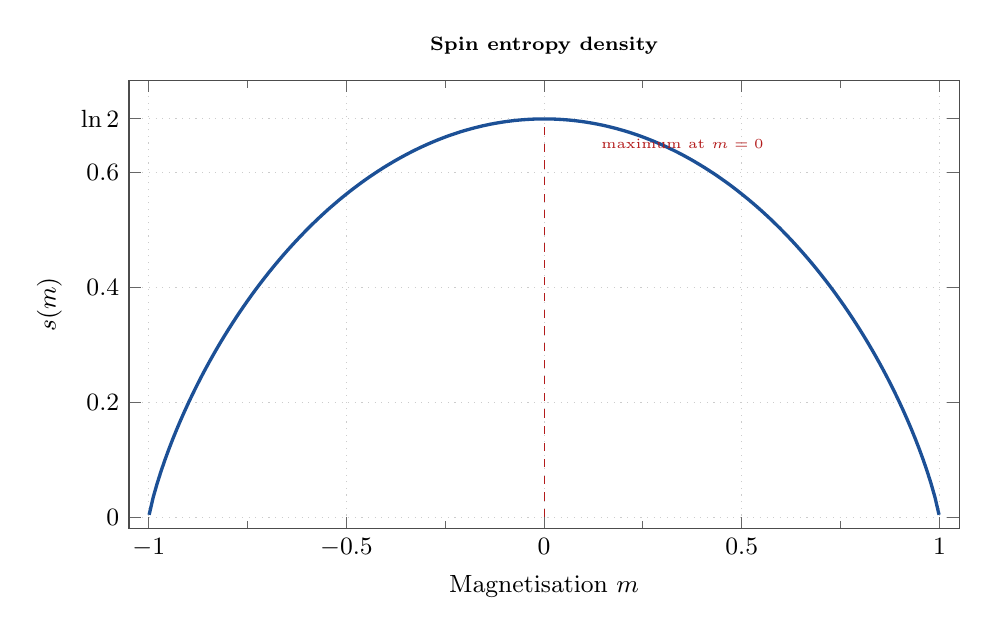
\begin{tikzpicture}
\begin{axis}[
  tufte axis,
  width=\linewidth, height=0.6\linewidth,
  xlabel={Magnetisation $m$},
  ylabel={$s(m)$},
  xmin=-1.05, xmax=1.05,
  ymin=-0.02, ymax=0.76,
  xtick={-1,-0.5,0,0.5,1},
  ytick={0,0.2,0.4,0.6,0.6931},
  yticklabels={0,0.2,0.4,0.6,$\ln 2$},
  title={\scriptsize Spin entropy density},
]
\addplot[tufteblue,very thick,domain=-0.999:0.999,samples=200]
  {-0.5*(1+x)*ln(0.5*(1+x)) - 0.5*(1-x)*ln(0.5*(1-x))};
\addplot[tuftered,dashed,thin] coordinates {(0,0)(0,0.6931)};
\node[font=\tiny,tuftered] at (axis cs:0.35,0.65){maximum at $m=0$};
\end{axis}
\end{tikzpicture}
\caption{The spin entropy density $s(m)$ from Eq.~\eqref{eq:spin_entropy}. It is maximised at $m=0$ (maximum disorder, $s=\log 2$) and vanishes at $m=\pm 1$ (all spins aligned).}
\label{fig:spin_entropy}
\end{figure}

% ============================================================
\section{Hubbard--Stratonovich transformation}
\label{sec:HS}
% ============================================================

\newthought{The Hubbard--Stratonovich (HS) transformation} is the central algebraic trick of mean-field theory. It converts an intractable quadratic coupling between many degrees of freedom into an integral over a single auxiliary field, making the saddle-point approximation applicable.

\subsection{The basic identity}

\begin{keyresult}
\begin{equation}
  e^{\frac{a^2}{2}}=\frac{1}{\sqrt{2\pi}}\int_{-\infty}^{\infty}\d z\; e^{-\frac{z^2}{2}+az}.
  \label{eq:HS_1d}
\end{equation}
\end{keyresult}

\noindent\textbf{Proof.} Complete the square in $z$: $-\frac{z^2}{2}+az=-\frac{1}{2}(z-a)^2+\frac{a^2}{2}$. Then:
\begin{align}
  \frac{1}{\sqrt{2\pi}}\int e^{-\frac{z^2}{2}+az}\d z
  &=\frac{e^{a^2/2}}{\sqrt{2\pi}}\int e^{-\frac{(z-a)^2}{2}}\d z
  =\frac{e^{a^2/2}}{\sqrt{2\pi}}\cdot\sqrt{2\pi}=e^{a^2/2}.\quad\checkmark
\end{align}

\subsection{General rescaled form}

For $\alpha>0$ and coupling $J$, substituting $a=J/\sqrt{\alpha}$ and $z\to\sqrt{\alpha}w$ in~\eqref{eq:HS_1d}:
\begin{keyresult}
\begin{equation}
  e^{\frac{J^2}{2\alpha}}=\sqrt{\frac{\alpha}{2\pi}}\int_{-\infty}^{\infty}\d z\; e^{-\frac{\alpha}{2}z^2+Jz}.
  \label{eq:HS_general}
\end{equation}
\end{keyresult}

\noindent\textbf{Derivation.} Start from~\eqref{eq:HS_1d} with $a=J/\sqrt{\alpha}$. Substitute $z=\sqrt{\alpha}\,w$:
\begin{equation}
  e^{\frac{J^2}{2\alpha}}
  =\frac{1}{\sqrt{2\pi}}\int e^{-\frac{z^2}{2}+\frac{Jz}{\sqrt{\alpha}}}\d z
  =\frac{\sqrt{\alpha}}{\sqrt{2\pi}}\int e^{-\frac{\alpha w^2}{2}+Jw}\d w.
\end{equation}

\subsection{Decoupling pairwise interactions}

The key application: a Boltzmann weight $e^{\frac{\beta J}{2N}(\sum_i\sigma_i)^2}$ couples every pair of spins. Setting $\alpha=N\beta J$ and $J_\text{eff}=\beta J\sum_i\sigma_i$ in~\eqref{eq:HS_general}:
\begin{keyresult}
\begin{equation}
  e^{\frac{\beta J}{2N}\left(\sum_i\sigma_i\right)^2}
  =\sqrt{\frac{N\beta J}{2\pi}}\int\d m\;\exp\!\left(-\frac{N\beta J}{2}m^2+\beta Jm\sum_{i=1}^N\sigma_i\right).
  \label{eq:HS_decouple}
\end{equation}
\end{keyresult}
After this transformation the exponent is \emph{linear} in each $\sigma_i$: the spins see only the uniform external field $\beta Jm$ and are completely decoupled from one another.

\begin{figure}
\centering
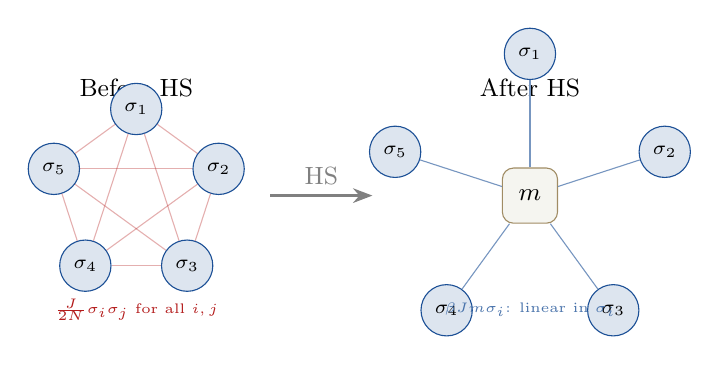
\begin{tikzpicture}[
  spin/.style={circle,draw=tufteblue,fill=tufteblue!15,minimum size=0.55cm,font=\scriptsize},
  arr/.style={{Stealth[length=4pt]}-{Stealth[length=4pt]},thick,tuftered!70},
  snarr/.style={{Stealth[length=4pt]}-,thick,black!50},
]
% ---- Left: all-to-all coupling ----
\begin{scope}
\node[font=\small,anchor=north] at (1.3,0.4) {Before HS};
\foreach \i/\a in {1/90,2/18,3/306,4/234,5/162}{
  \node[spin] (L\i) at ({1.3+1.1*cos(\a)},{1.1*sin(\a)-1.2}) {$\sigma_{\i}$};
}
\foreach \i in {1,...,5}{
  \foreach \j in {1,...,5}{
    \ifnum\i<\j
      \draw[tuftered,opacity=0.35,thin] (L\i) -- (L\j);
    \fi
  }
}
\node[font=\tiny,tuftered] at (1.3,-2.65) {$\frac{J}{2N}\sigma_i\sigma_j$ for all $i,j$};
\end{scope}

% ---- Arrow ----
\draw[-{Stealth[length=7pt]},very thick,black!50]
  (3.0,-1.2) -- node[above,font=\small]{HS} (4.3,-1.2);

% ---- Right: auxiliary field coupling ----
\begin{scope}[xshift=5.0cm]
\node[font=\small,anchor=north] at (1.3,0.4) {After HS};
% auxiliary field node
\node[draw=resultframe,fill=resultbox,rounded corners=4pt,
      minimum size=0.7cm,font=\small] (m) at (1.3,-1.2) {$m$};
\foreach \i/\a in {1/90,2/18,3/306,4/234,5/162}{
  \node[spin] (R\i) at ({1.3+1.8*cos(\a)},{1.8*sin(\a)-1.2}) {$\sigma_{\i}$};
  \draw[tufteblue!60,thin] (m) -- (R\i);
}
\node[font=\tiny,tufteblue!80] at (1.3,-2.65) {$\beta Jm\sigma_i$: linear in $\sigma_i$};
\end{scope}
\end{tikzpicture}
\caption{The Hubbard--Stratonovich transformation. Left: the original problem has all-to-all quadratic interactions $J\sigma_i\sigma_j/2N$, making the partition function a sum of $2^N$ entangled terms. Right: after introducing the auxiliary field $m$, each spin interacts only with $m$ through a \emph{linear} coupling $\beta Jm\sigma_i$; the spins decouple and the sum factorises.}
\label{fig:HS_diagram}
\end{figure}

\subsection{Application: Curie--Weiss mean-field theory}

\newthought{The Curie--Weiss model} is the fully-connected Ising model:
\begin{equation}
  H=-\frac{J}{2N}\sum_{i,j}\sigma_i\sigma_j
   =-\frac{J}{2N}\!\left(\sum_i\sigma_i\right)^2,\quad \sigma_i\in\{+1,-1\}.
\end{equation}
The partition function is $Z=\sum_{\{\sigma_i\}}e^{-\beta H}$.

\textbf{Step 1 — Apply HS.}
\begin{equation}
  Z=\sqrt{\frac{N\beta J}{2\pi}}\int\d m\;e^{-\frac{N\beta J}{2}m^2}
    \sum_{\{\sigma_i\}}\prod_{i=1}^N e^{\beta Jm\sigma_i}.
\end{equation}

\textbf{Step 2 — Factorise.} Spins are independent after HS:
\begin{equation}
  \sum_{\{\sigma_i\}}\prod_i e^{\beta Jm\sigma_i}
  =\prod_i(e^{\beta Jm}+e^{-\beta Jm})=(2\cosh\beta Jm)^N.
\end{equation}

\textbf{Step 3 — Write as single integral.}
\begin{equation}
  Z=\sqrt{\frac{N\beta J}{2\pi}}\int\d m\;\exp\!\bigl(-Nf(m)\bigr),
  \quad f(m)=\tfrac{\beta J}{2}m^2-\log(2\cosh\beta Jm).
\end{equation}

\textbf{Step 4 — Saddle-point.} $f'(m^*)=\beta J[m^*-\tanh(\beta Jm^*)]=0$:
\begin{keyresult}
\begin{equation}
  m^*=\tanh(\beta J m^*).
  \label{eq:CW_self_consistency}
\end{equation}
\end{keyresult}
This is the \textbf{mean-field self-consistency equation}. The auxiliary field $m$ is the magnetisation $m^*=\langle\sigma_i\rangle$.

\textbf{Step 5 — Phase structure.} Non-trivial solutions $m^*\neq 0$ require the slope of $\tanh(\beta Jm)$ at $m=0$ to exceed 1:
\begin{equation}
  \beta J>1 \quad\Longleftrightarrow\quad T<T_c\equiv J.
\end{equation}

\begin{figure}
\centering
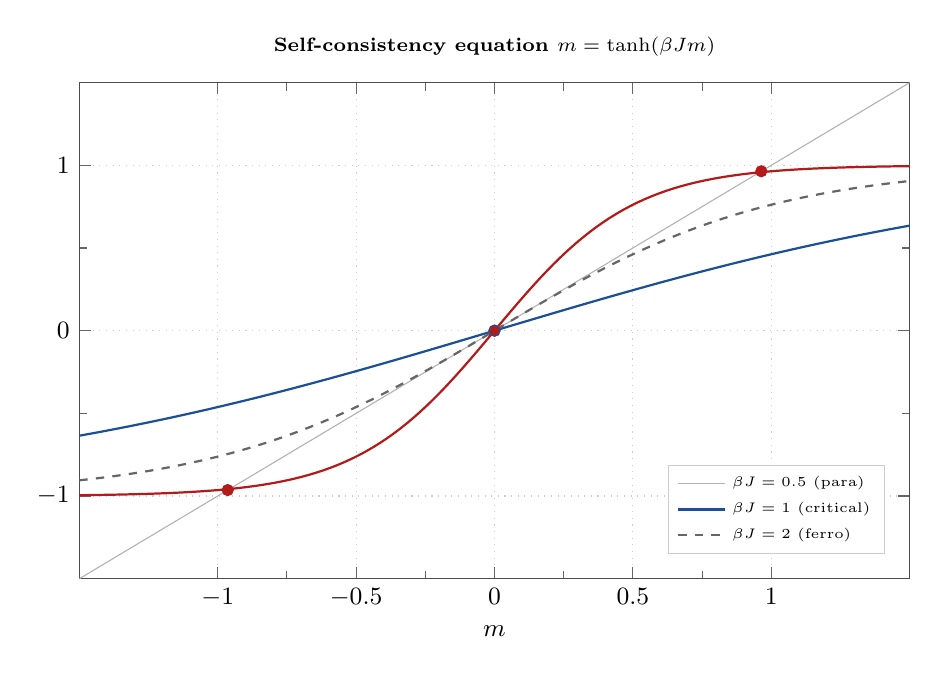
\begin{tikzpicture}
\begin{axis}[
  tufte axis,
  width=\linewidth, height=0.65\linewidth,
  xlabel={$m$},
  ylabel={},
  xmin=-1.5, xmax=1.5,
  ymin=-1.5, ymax=1.5,
  xtick={-1,-0.5,0,0.5,1},
  ytick={-1,0,1},
  title={\scriptsize Self-consistency equation $m=\tanh(\beta J m)$},
  legend style={at={(0.97,0.05)},anchor=south east,font=\tiny,
                draw=black!20,fill=white},
  legend cell align=left,
]
% diagonal m = m
\addplot[black!30,thin,domain=-1.5:1.5]{x};
% subcritical beta*J = 0.5
\addplot[tufteblue,thick,domain=-1.5:1.5,samples=120]
  {tanh(0.5*x)};
\addlegendentry{$\beta J=0.5$ (para)};
% critical beta*J = 1
\addplot[black!60,thick,dashed,domain=-1.5:1.5,samples=120]
  {tanh(1.0*x)};
\addlegendentry{$\beta J=1$ (critical)};
% supercritical beta*J = 2
\addplot[tuftered,thick,domain=-1.5:1.5,samples=120]
  {tanh(2.0*x)};
\addlegendentry{$\beta J=2$ (ferro)};
% fixed points for beta*J=2
\addplot[tuftered,only marks,mark=*,mark size=2pt]
  coordinates {(0,0)(0.9640,0.9640)(-0.9640,-0.9640)};
\addplot[tufteblue,only marks,mark=o,mark size=2pt]
  coordinates {(0,0)};
\end{axis}
\end{tikzpicture}
\caption{Graphical solution of the self-consistency equation~\eqref{eq:CW_self_consistency}. Intersections of $y=\tanh(\beta Jm)$ with the diagonal $y=m$ give the solutions $m^*$. Below $T_c$ ($\beta J>1$, red curve) three intersections appear: $m^*=0$ (unstable) and $m^*=\pm m_0$ (stable, filled dots). Above $T_c$ ($\beta J<1$, blue) only $m^*=0$ exists.}
\label{fig:CW_bifurcation}
\end{figure}

Above $T_c$ only the paramagnetic solution $m^*=0$ exists. Below $T_c$ two ferromagnetic solutions $m^*=\pm m_0$ appear — this is the \textbf{ferromagnetic phase transition}, illustrated in Figure~\ref{fig:CW_bifurcation}. The entire derivation (HS $\to$ spin factorisation $\to$ saddle-point $\to$ self-consistency equation) is the prototype for every mean-field calculation in this course, including the Hopfield model and the replica method.

\end{document}